
\begin{frame}
    \frametitle{Verzování - kód}

    Verzování kódu nám umožňuje:
    \begin{itemize}
        \item Uchovávat historii změn
        \item Spolupracovat na kódu
        \item Zpětně se vracet ke starším verzím v případě chyby
    \end{itemize}
\end{frame}

\begin{frame}
    \frametitle{Verzování - Git}

    \onslide<1->{
        K verzování kódu knihovny jsem zvolil nástroj Git s webovou službou GitHub.\\
    }
    \onslide<2->{
        Tuto kombinaci jsem zvolil převážně protože:
        \begin{itemize}
            \item Git je zdaleka nejpoužívanější nástroj pro verzování kódu na světě
            \item GitHub nabízí výhodné podmínky pro open-source projekty a vše, co potřebuji, je zdarma
            \item Projekt je snadno vyhledatelný a má přehlednou stránku repozitáře přímo na GitHubu
        \end{itemize}
    }
\end{frame}

\begin{frame}
    \frametitle{Verzování - Stránka projektu na GitHubu}
    \framesubtitle{Hlavní stránka projektu}
    \begin{figure}
        \centering
        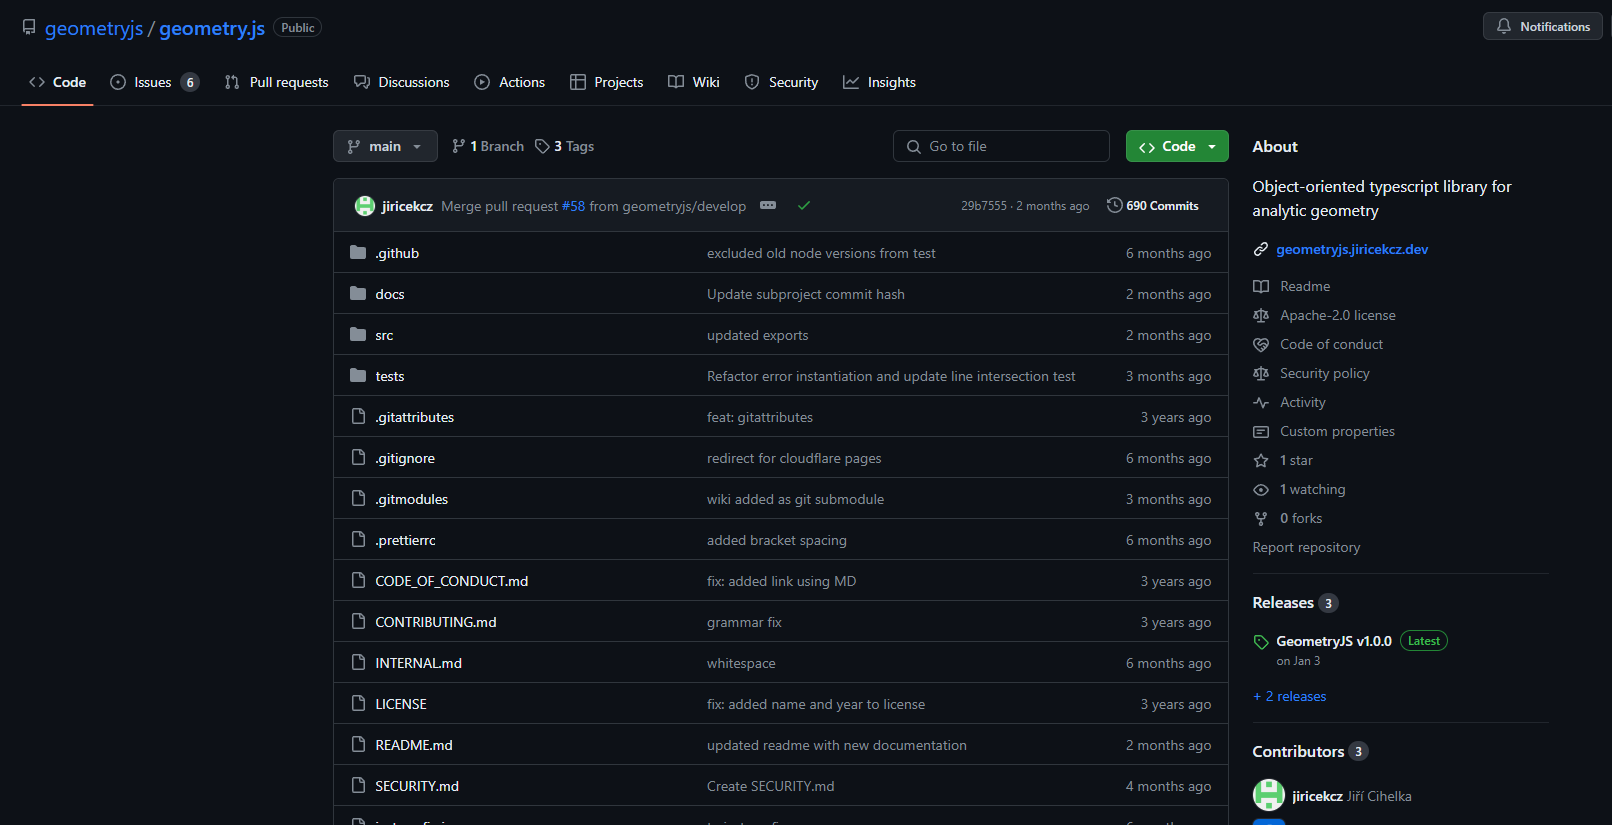
\includegraphics[height=0.665\textheight]{../resources/github-page.png}
        \caption{Ukázka repozitáře na GitHubu}
    \end{figure}
\end{frame}

\begin{frame}
    \frametitle{Verzování - Stránka projektu na GitHubu}
    \framesubtitle{Issues na GitHubu}
    \begin{figure}
        \centering
        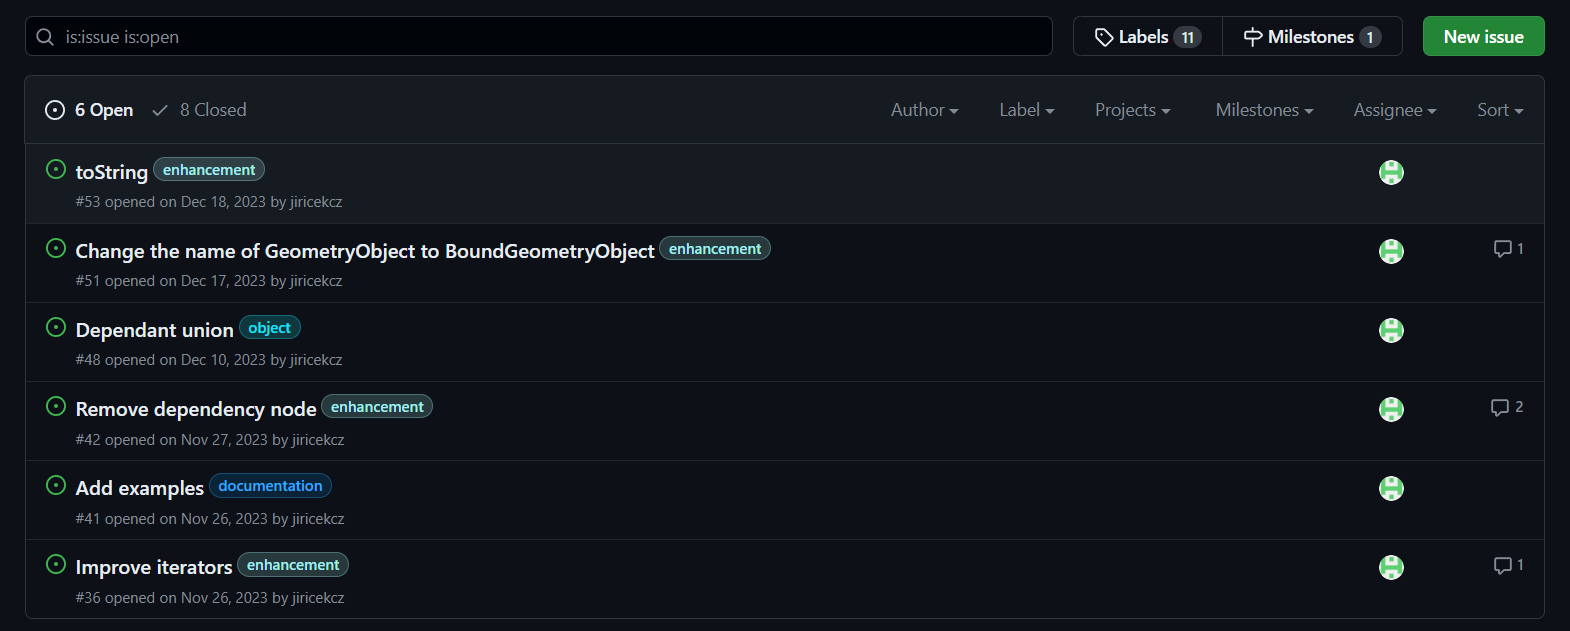
\includegraphics[height=0.60\textheight]{../resources/github-issues.png}
        \caption{Ukázka správy issues na GitHubu}
    \end{figure}
\end{frame}

\begin{frame}
    \frametitle{Verzování - Stránka projektu na GitHubu}
    \framesubtitle{Historie commitů}
    \begin{figure}
        \centering
        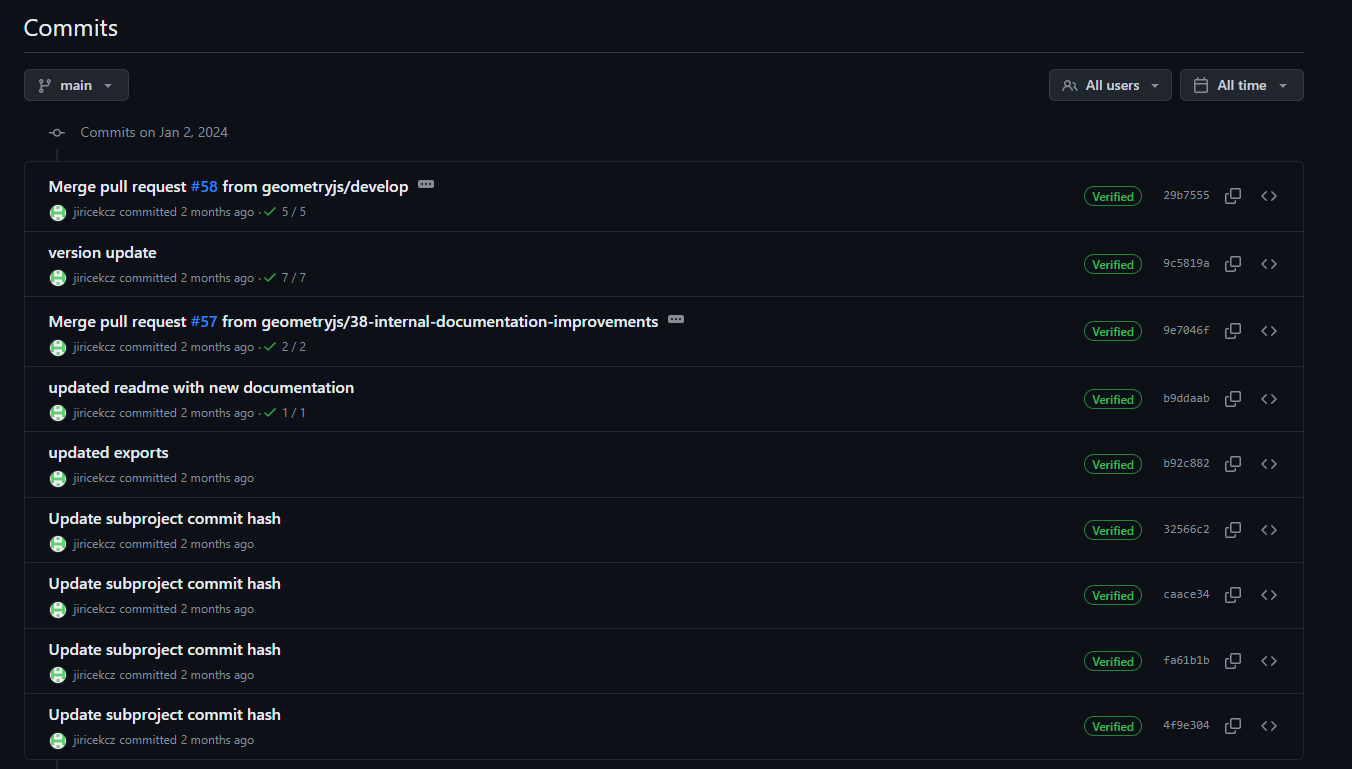
\includegraphics[height=0.665\textheight]{../resources/github-commits.png}
        \caption{Ukázka historie commitů na GitHubu}
    \end{figure}
\end{frame}


\begin{frame}
    \frametitle{Verzování - Vydání}
    \begin{definition}[Vydání]
        \textbf{Vydání} (release) je označení určité verze kódu.
    \end{definition}

    \begin{block}{Číslování vydání}
        Standardní způsob číslování vydání je pomocí tzv. \textbf{Semantic Versioning}\cite{semantic_versioning:2.0.0} \\
        Zjednodušeně: \texttt{MAJOR.MINOR.PATCH}
    \end{block}
\end{frame}

\begin{frame}
    \frametitle{Verzování - Ukázka vydání}
    \begin{figure}
        \centering
        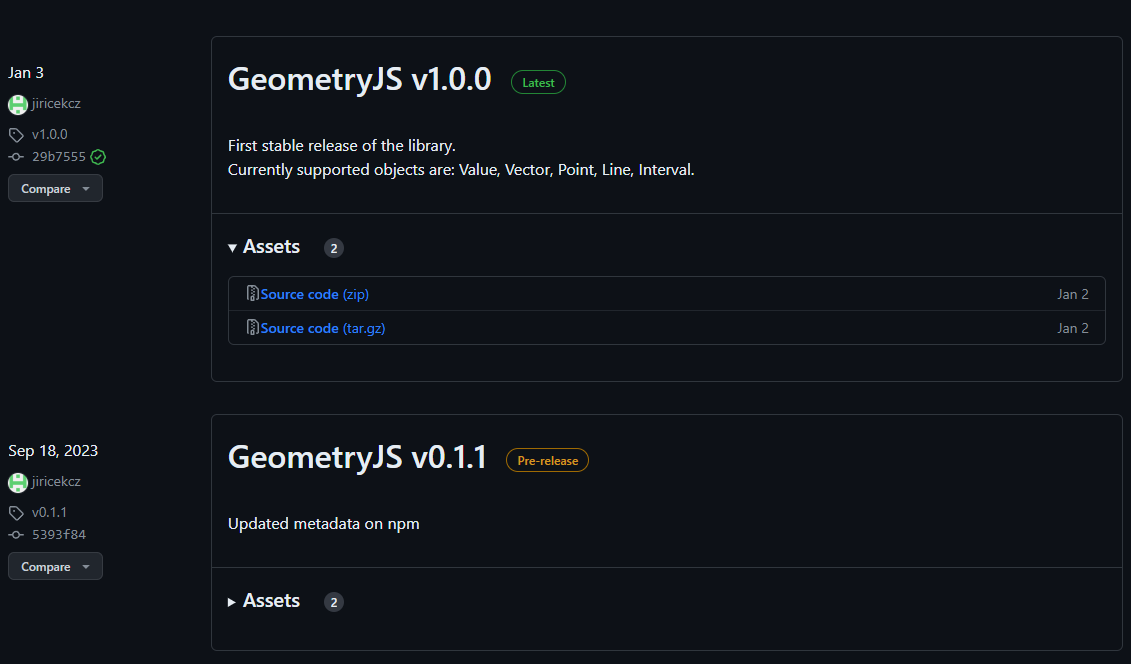
\includegraphics[height=0.7\textheight]{../resources/github-releases.png}
        \caption{Ukázka vydání na GitHubu}
    \end{figure}
\end{frame}